% \usepackage{tikz}

% \begin{tikzpicture}[
%     font=\sffamily,
%     every matrix/.style={ampersand replacement=\&,column sep=2cm, row sep=2cm},
%     source/.style={draw, thick, rounded corners, fill=yellow!20, inner sep=.3cm},
%     process/.style={draw, thick, cirlce, fill=blue!20},
%     sink/.style={source, fill=green!20},
%     dots/.style={gray, scale=2},
%     to/.style={->,>=stealth',shorten >= 1pt, semithick, font=\sffamily\footnotesize},
%     every node/.style={align=center}
% ]
%     \matrix{
%         \node[]}
% \end{tikzpicture}


\chapter{Tikz}
This section introduce how to use tika package to produce wanted plots.

%%%%%%%%%%%%%%%%%%%%%%%%%%%%%%%%%%%%%%%%%%%%%%%%
\subsection{Simple shapes}

%%%%%%%%%%%%%%%%%%%%%%%%
\subsubsection{coordinate}
Coordinates can be specified in round brackets in an arbitrary TEX 
dimension either using Cartesion coordinates (comma separated), e.g. 
1cm in the x direction and 2pt in the y direction
\begin{tcolorbox}
\textsc{1cm, 2pt}
\end{tcolorbox}
\tikz\draw (0,0)--(0,2)--(2,0)--(0,0);


%%%%%%%%%%%%%%%%%%%%%%%%
\subsubsection{circle and ellipse}
\tikz\draw[line width=2mm, color=black] (0,0) circle (4ex);
\tikz\draw[fill=gray!30!white](0,0) ellipse (20pt and 28pt);
\tikz\draw[fill=gray!60!white] (0,0) ellipse (28pt and 20pt);

%%%%%%%%%%%%%%%%%%%%%%%%
\subsubsection{rectangle}
\begin{tikzpicture}
    \coordinate (O) (2,2);
    \node[draw, rectangle] (rec) at (0,0) {rectangle};	% here the coordinate (0,0) is the bottom left point's coor.
    \draw[thick] (O) rectangle ++(2,1);
\end{tikzpicture}
\begin{tikzpicture}
    \coordinate (O) (2,2);
    \node[draw, rectangle] (rec) at (0,0) {rectangle};	
    \draw[thick] (O) rectangle (2,1);
\end{tikzpicture}
\begin{tikzpicture}
    \node[draw, rectangle] (rec) at (0,0) {rectangle};	
    \draw[thick] (2,2) rectangle (2,1);
\end{tikzpicture}
\begin{tikzpicture}
    \node[draw, rectangle] (rec) at (0,0) {rectangle};	
    \draw[thick] (2,2) rectangle ++(2,1);
\end{tikzpicture}
The \emph{rectangle} command requires the absolute corner coords. 
You are giving the increments in the second coordinates. So we can see
in the third above plot, it looks like a line, because the second coordinate
is not given as increments.

%%%%%%%%%%%%%%%%%%%%%%%%
\subsubsection{grid}
\begin{tikzpicture}
    \draw[step=0.25cm,gray,thick](-1,-1) grid(1,1);
\end{tikzpicture}

%%%%%%%%%%%%%%%%%%%%%%%%
\subsubsection{parabola, sin, cos}
\begin{tikzpicture}
    \draw (-1.5, 0) -- (1.5, 0);
    \draw (0, -1.5) -- (0, 1.5);
    \draw (0, 0) circle (.8cm);
    \draw (-1, -1) rectangle (1, 1);
    \draw[gray] (-.5, -.5) parabola (1, 1);
\end{tikzpicture}
\tikz\draw[x=5pt, y=5pt] (0,0) parabola bend (4,16) (6,12);

{\bf sin} and {\bf cos} add a sine or cosine curve in the interval 
[0, $\pi/2$] such that the previous current point is at the start of the
curve and the curve ends at the given end point following it.

\tikz\draw[x=10pt,y=10pt] (0,0) sin (1,1) cos (2,0) sin (3,-1) cos (4,0)
			  (0,1) cos (1,0) sin (2,-1) cos (3,0) sin (4,1);
%%%%%%%%%%%%%%%%%%%%%%%%
\subsubsection{arc}
\begin{tikzpicture}
    \draw (-.5, 0) -- (1.5, 0);
    \draw (0, -.5) -- (0, 1.5);
    \draw (1, 0) arc (-25:70:1cm);
    \draw[gray] (-.5, -.5) parabola (1, 1);
\end{tikzpicture}
\hfill
\tikz\draw (0,0) arc (0:180:1cm);
\hfill
\hfill
\tikz\draw[fill=gray!50] (4, 0) -- +(30:1cm) arc (30:60:1cm) -- cycle;
\hfill
\tikz\draw[fill=gray!50] (4, 0) -- +(30:2cm) arc (30:60:1cm) -- cycle;

\begin{tikzpicture}
    \draw (0,1) arc (90:270:1);
    \draw (1,0) arc (-90:90:1);
    \draw (3,1) arc (90:270:0.3 and 1);
    \draw (3,1) arc (90:270:0.5 and 1);
    \draw (0,0) arc (0:315:1.75cm and 1cm);
\end{tikzpicture}


%%%%%%%%%%%%%%%%%%%%%%%%
\subsubsection{Arrow}
To draw the arrow head whthin the line, use \emph{decorate} option. \\
(need \verb|\usetikzlibrary{decorations.markings}|)

\begin{tikzpicture}
    \tikzstyle arrowstyle=[scale=1]
    \tikzstyle directed=[postaction={decorate,decoration={markings,
    mark=at position .65 with {\arrow[arrowstyle]{stealth}}}}]
    \tikzstyle reversed directed=[postaction={decorate, decoration={markings,
    mark=at position .65 with {\arrowreversed[arrowstyle]{stealth}}}}]

    \draw [red, ultra thick, directed] (0,0) -- (2,2);
\end{tikzpicture}

%%%%%%%%%%%%%%%%%%%%%%%%
\subsubsection{control points}
Control points in drawing.

\hfill
\begin{tikzpicture}
    \fill[GreenYellow!35] (-5pt, -5pt) rectangle (2cm+5pt, 2cm+5pt);

    \filldraw [gray] (0,0) circle (2pt)
		     (1,1) circle (2pt)
		     (2,1) circle (2pt)
		     (2,0) circle (2pt);
    \draw (0,0) .. controls (1,1) and (2,1) .. (2,0);

    \footnotesize
    \draw[shift={(2,1)}, xshift=0.5cm]
    node [right, text width=12cm, rounded corners, fill=blue!20,inner sep=1ex]
    {
	\begin{lstlisting}[language=TeX]
\begin{tikzpicture}
    \filldraw [gray] (0,0) circle (2pt)
		     (1,1) circle (2pt)
		     (2,1) circle (2pt)
		     (2,0) circle (2pt);
    \draw (0,0) .. controls (1,1) and (2,1) .. (2,0);
\end{tikzpicture}
	\end{lstlisting}
    };
\end{tikzpicture}

\hfill
\begin{tikzpicture}
    \fill[GreenYellow!35] (-1.5cm-5pt, -1.5cm-5pt) rectangle (1.5cm+5pt, 1.5cm+5pt);

    \draw (-1.5,0) -- (1.5,0);
    \draw (0,-1.5) -- (0,1.5);
    \draw (-1,0) .. controls (-1,0.555) and (-0.555,1) .. (0,1)
		 .. controls (0.555,1) and (1,0.555) .. (1,0);

    \footnotesize
    \draw[shift={(1.5,0)}, xshift=0.5cm]
    node [right, text width=12cm, rounded corners, fill=blue!20,inner sep=1ex]
    {
	\begin{lstlisting}[language=TeX]
\begin{tikzpicture}
    \draw (-1.5,0) -- (1.5,0);
    \draw (0,-1.5) -- (0,1.5);
    \draw (-1,0) .. controls (-1,0.555) and (-0.555,1) .. (0,1)
		 .. controls (0.555,1) and (1,0.555) .. (1,0);
\end{tikzpicture}
	\end{lstlisting}
    };
\end{tikzpicture}

\begin{tikzpicture}[scale=3]
    \fill[GreenYellow!35] (-.1cm-5pt, -.2cm-5pt) rectangle (1.1cm+5pt, 0.75cm+5pt);

    \clip (-0.1,-0.2) rectangle (1.1,0.75);
    \draw[step=.5cm,gray,very thin] (-1.4,-1.4) grid (1.4,1.4);
    \draw (-1.5,0) -- (1.5,0);
    \draw (0,-1.5) -- (0,1.5);
    \draw (0,0) circle (1cm);
    \draw (3mm,0mm) arc (0:30:3mm);
\end{tikzpicture}

If you use relative control points, then the first one is relative to the
start node, while the second one is relative to the end node.

%%%%%%%%%%%%%%%%%%%%%%%%
\subsubsection{shade}
\verb|\shade| and \verb|\shadedraw|

\tikz \shade (0,0) rectangle (2,1)  (3,0.5) circle (0.5cm);

The default shading is a smooth transition from gray to white. To use 
other colors, specify them in options:

\begin{tikzpicture}[rounded corners, ultra thick]
    \shade [top color=yellow, bottom color=black] (0,0) rectangle +(2,1);
    \shade [left color=yellow, right color=black] (3,0) rectangle +(2,1);
    \shade [inner color=yellow, outer color=black, draw=yellow] (6,0) rectangle +(2,1);
    \shade [ball color=green] (9,.5) circle (0.5cm);
\end{tikzpicture}

%%%%%%%%%%%%%%%%%%%%%%%%
\subsubsection{+ sign}
\verb|+(1cm,0cm)| means ``1cm upwards from the previous specified position"; 
while \verb|++(0cm,2cm)| means ``2cm to the right of the previous specified
position, making this the {\bf new} specified position."

\tcbset{colback=brown!30}
\begin{tcolorbox}[width=4cm]
    \begin{tikzpicture}[scale=3]
	\clip (-0.1,-0.2) rectangle (1.1,0.75);
	\draw[step=.5cm,gray,very thin] (-1.4,-1.4) grid (1.4,1.4);
	\draw (-1.5,0) -- (1.5,0);
	\draw (0,-1.5) -- (0,1.5);
	\draw (0,0) circle (1cm);
	\draw (3mm,0mm) arc (0:30:3mm);
	\filldraw[fill=green!20,draw=green!50!black] (0,0) -- (3mm,0mm) arc (0:30:3mm) -- cycle;
	\draw[red,very thick] (30:1cm) -- +(0,-0.5);
	\draw[blue,very thick] (30:1cm) ++(0,-0.5) -- (0,0);
\end{tikzpicture}
\end{tcolorbox}

Note the difference between \verb|+| and \verb|++| (see the code).

Using \verb|++|:
\begin{tikzpicture}
    \def\rectanglepath{-- ++(1,0) -- ++(0,1) -- ++(-1,0) -- cycle}
    \draw (0,0) \rectanglepath;
    \draw (1.5,0) \rectanglepath;
\end{tikzpicture}

Using \verb|+|:
\begin{tikzpicture}
    \def\rectanglepath{-- +(1,0) -- +(1,1) -- +(0,1) -- cycle}
    \draw (0,0) \rectanglepath;
    \draw (1.5,0) \rectanglepath;
\end{tikzpicture}

%%%%%%%%%%%%%%%%%%%%%%%%
\subsubsection{Intersection}
\verb/(<p> |- <q>)/ is ``the intersection of a vertical line through p and a horizontal line through q."

An intersection between a line going up from (1,0) and aline going from 
the origin throught (30:1cm).

\tcbset{colback=blue!20}
\begin{tcolorbox}
    \verb|\draw[very thick,orange] (1,0) -- (intersection of 1,0--1,1 and 0,0--30:1cm);|
\end{tcolorbox}

%%%%%%%%%%%%%%%%%%%%%%%%
\subsubsection{Miscellaneous}
\begin{tikzpicture}[line width=5pt]
    \draw (0,0) -- (1,0) -- (1,1) -- (0,0);
    \draw (2,0) -- (3,0) -- (3,1) -- cycle;
    \useasboundingbox (0,1.5);
\end{tikzpicture}
%%%%%%%%%%%%%%%%%%%%%%%%%%%%%%%%%%%%%%%%%%%%%%%%
\subsection{Coordinate Systems}
\begin{itemize}
    \item canvas
    \item xyz
    \item canvas polar
    \item xyz polar
    \item barycentric
	\[
	    {\alpha_1\vec{v}_1 + \alpha_2\vec{v}_2 + \cdots + \alpha_n\vec{v}_n} \over {\alpha_1 + \alpha_2 + \cdots + \alpha_n}
	    \]
    \item node
    \item intersection
    \item perpendicular
\end{itemize}
Any {\bf canvas} coordinate system requires explict dimensions (units)
while {\bf xyz} coordinate systems don't.

e.g.

\hfill
\begin{tikzpicture}
    \fill[GreenYellow!40] (-5pt,-5pt) rectangle (2cm + 5pt, 2cm + 5pt);

    \draw [help lines] (0,0) grid (2,2);

    \draw (0,0) -- (canvas polar cs:angle=30,radius=1cm);
    \draw (0,0) -- (xyz polar cs:angle=60, radius=1);

    \footnotesize
    \draw[shift={(2,1)},xshift=0.5cm]
    node [right, text width=12cm, rounded corners, fill=blue!20,inner sep=1ex]
    {
	\begin{lstlisting}[language=TeX]
\begin{tikzpicture}
  \draw [help lines] (0,0) grid (2,2);
  
  \draw (0,0) -- (canvas polar cs:angle=30,radius=1cm);
  \draw (0,0) -- (xyz polar cs:angle=60, radius=1);
\end{tikzpicture}
	\end{lstlisting}
    };
\end{tikzpicture}

\subsection{Options}
%%%%%%%%%%%%%%%%%%%%%%%%
\subsubsection{line width}
\tikz\draw[line width=2mm] (0,0)--(4,0);
\subsubsection{rotate}
\tikz\draw[rotate=45] (0,0) ellipse (16pt and 20pt);
\subsubsection{scale}
\tikz\draw[scale=1.5,rotate=75] (0,0) ellipse (10pt and 16pt);
\subsubsection{xscale, yscale}
\tikz\draw[xscale=1.5, yscale=0.5] (0,0) ellipse (10pt and 16pt);


%%%%%%%%%%%%%%%%%%%%%%%%%%%%%%%%%%%%%%%%%%%%%%%%
\subsection{node}
\tikz\draw(1,1) node{A} -- (2,2) node{B};
\hfill
\tikz\draw(1,1) node[circle, draw]{A} -- (2,2) node[circle,draw]{B};

%%%%%%%%%%%%%%%%%%%%%%%%
\subsubsection{label and pin}
\tikz[label distance=2mm]
\node[circle,fill=gray!45,label=above:12,label=right:3,label=below:6,label=left:9]{clock};
\hfill
\tikz[pin distance=4mm]\draw(1,1)
node[circle,fill=gray!45,pin=above:12,pin=right:3,pin=below:6,pin=left:9]{}
circle (1cm);

%%%%%%%%%%%%%%%%%%%%%%%%%%%%%%%%%%%%%%%%%%%%%%%%
\subsection{Styles}
tikzstyle:
\begin{itemize}
    \item every path
    \item every node
	\begin{itemize}
	    \item every \textless {\it shape} \textgreater node
	    \item every \textless {\it part name} \textgreater node part
	    \item every label
	    \item every pin
	    \item every pin edge
	\end{itemize}
    \item every to
    \item every curve
    \item every line
    \item every edge
    \item every snake
    \item every matrix
	\begin{itemize}
	    \item every cell
	\end{itemize}
    \item tree
	\begin{itemize}
	    \item every child
	    \item every child node
	    \item level \textless {\it number} \textgreater
	\end{itemize}
    \item every plot
\end{itemize}
When defining tikzstyle, there is no space allowed between the defined style and the definition.

\verb|\tikzstyle arrowstyle=[scale=1]|	\textbf{Corrected}. \\
\verb|\tikzstyle arrowstyle = [scale=1]|\textit{Wrong}.
%%%%%%%%%%%%%%%%%%%%%%%%%%%%%%%%%%%%%%%%%%%%%%%%
\subsection{plot}
%%%%%%%%%%%%%%%%%%%%%%%%
\subsubsection{gnuplot}
Tikz use \emph{gnuplot} to plot function, so to get right plot, we need to
install \emph{gnuplot} firstly. After first complining, we will get a
*.x.gnuplot file, run \emph{gnuplot} against this file, then compile tex
file again, we will get wanted plots.

difference between \verb|--plot| and \verb|plot|
\tikz\draw(0,1) -- (1,1) --plot coordinates {(2,0) (2, 1.5)};
\tikz\draw(0,1) -- (1,1) plot coordinates {(2,0) (2, 1.5)};

\begin{tikzpicture}[domain=0:2]
    \draw[thick,color=gray,step=0.5cm,dashed] (-0.5,-0.5) grid(3,3);
    \draw[->] (-1,0) -- (3.5,0) node[below right] {$x$};
    \draw[->] (0,-1) -- (0,3.5) node[left] {$y$};
    \draw plot[id=x] function{x*x};
\end{tikzpicture}

%%%%%%%%%%%%%%%%%%%%%%%%
\subsubsection{note on plots}
\begin{tikzpicture}
\node [anchor=west] (note) at (-1,3) {\Large Note};
\node [anchor=west] (water) at (-1,1) {\Large Water};
\begin{scope}[xshift=1.5cm]
    \node[anchor=south west,inner sep=0] (image) at (0,0)
    {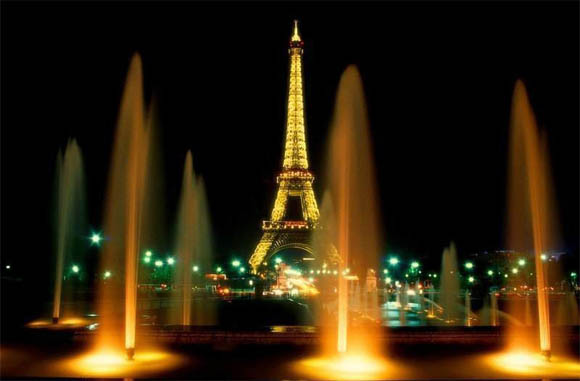
\includegraphics[width=0.7\textwidth]{eiffel.jpg}};
    \begin{scope}[x={(image.south east)},y={(image.north west)}]
        \draw[red,ultra thick,rounded corners] (0.48,0.80) rectangle (0.55,0.95);
        \draw [-latex, ultra thick, red] (note) to[out=0, in=-120] (0.48,0.80);
        \draw [-stealth, line width=5pt, cyan] (water) -- ++(0.4,0.0);
    \end{scope}
\end{scope}
\end{tikzpicture}

%%%%%%%%%%%%%%%%%%%%%%%%%%%%%%%%%%%%%%%%%%%%%%%%%%%%%%%%%%%%%%%%%%%%%%%%
\section{Examples}
\begin{tikzpicture}
    \begin{scope}[very thick,dashed]
	\draw (0,0) circle (.5cm);
	\draw (0,0) circle (1cm);
    \end{scope}
    \draw[thin] (0,0) circle (1.5cm);
\end{tikzpicture}
\hfill

\begin{tikzpicture}[scale=1]
    \pgfmathsetmacro{\minsize}{0.2cm}
    \pgfmathsetmacro{\nodedist}{3}  
    \newcommand{\fillcolor}{black}

    \tikzstyle{every node}=[draw,shape=circle,minimum size=\minsize,inner sep=0]
    \foreach \x in {0,...,5}
	\node[fill=\fillcolor] (p\x) at (\x*60:\nodedist) {};	% (angle:radius)
    \foreach \x in {0,...,4}
    {
	\pgfmathtruncatemacro{\startvalue}{\x+1}
	\foreach \y in {\startvalue,...,5}
	    \draw (p\x) -- (p\y);
    }
\end{tikzpicture}
\hfill

\begin{tikzpicture}
    \draw (-.5, 0)--(1.5,0);
    \draw (0, -.5)--(0, 1.5);
    \fill[gray] (0,0)--(1,0) arc (0:45:1cm) -- cycle;
    \draw[thin] (0,0) circle (1.5cm);
\end{tikzpicture}

\begin{tikzpicture}[node distance=2.8cm, auto]
    \tikzstyle{block}=[rectangle, draw, rounded corners, text width=2cm,
    text centered, fill=blue!30];
    \tikzstyle{cloud}=[ellipse, draw, fill=pink!50, text centered];
    \tikzstyle{decision}=[diamond, draw,aspect=1.5,text width=2cm,text centered];
    \tikzstyle{line}=[->,black,thick,draw];
    % Place nodes
    \node [block] (init) {initialize model};
    \node [cloud, left of=init] (expert) {expert};
    \node [cloud, right of=init] (system) {system};
    \node [block, below of=init] (identify) {identify candidate models};
    \node [block, below of=identify] (evaluate) {evaluate candidate models};
    \node [block, left of=evaluate, node distance=3cm] (update) {update model};
    \node [decision, below of=evaluate] (decide) {is best candidate better?};
    \node [block, below of=decide, node distance=3cm] (stop) {stop};
    % Draw edges
    \path [line] (init) -- (identify);
    \path [line] (identify) -- (evaluate);
    \path [line] (evaluate) -- (decide);
    \path [line] (decide) -| node [near start] {yes} (update);
    \path [line] (update) |- (identify);
    \path [line] (decide) -- node {no}(stop);
    \path [line,dashed] (expert) -- (init);
    \path [line,dashed] (system) -- (init);
    \path [line,dashed] (system) |- (evaluate);
\end{tikzpicture}
